\documentclass{standalone}
\usepackage{tikz}
\usetikzlibrary{patterns}
\usetikzlibrary{positioning}
\usetikzlibrary{patterns, positioning}
\usetikzlibrary{shapes.misc}
\usepackage[outline]{contour}
\contourlength{1.5pt} 
\usepackage[sfdefault]{ClearSans}

\begin{document}
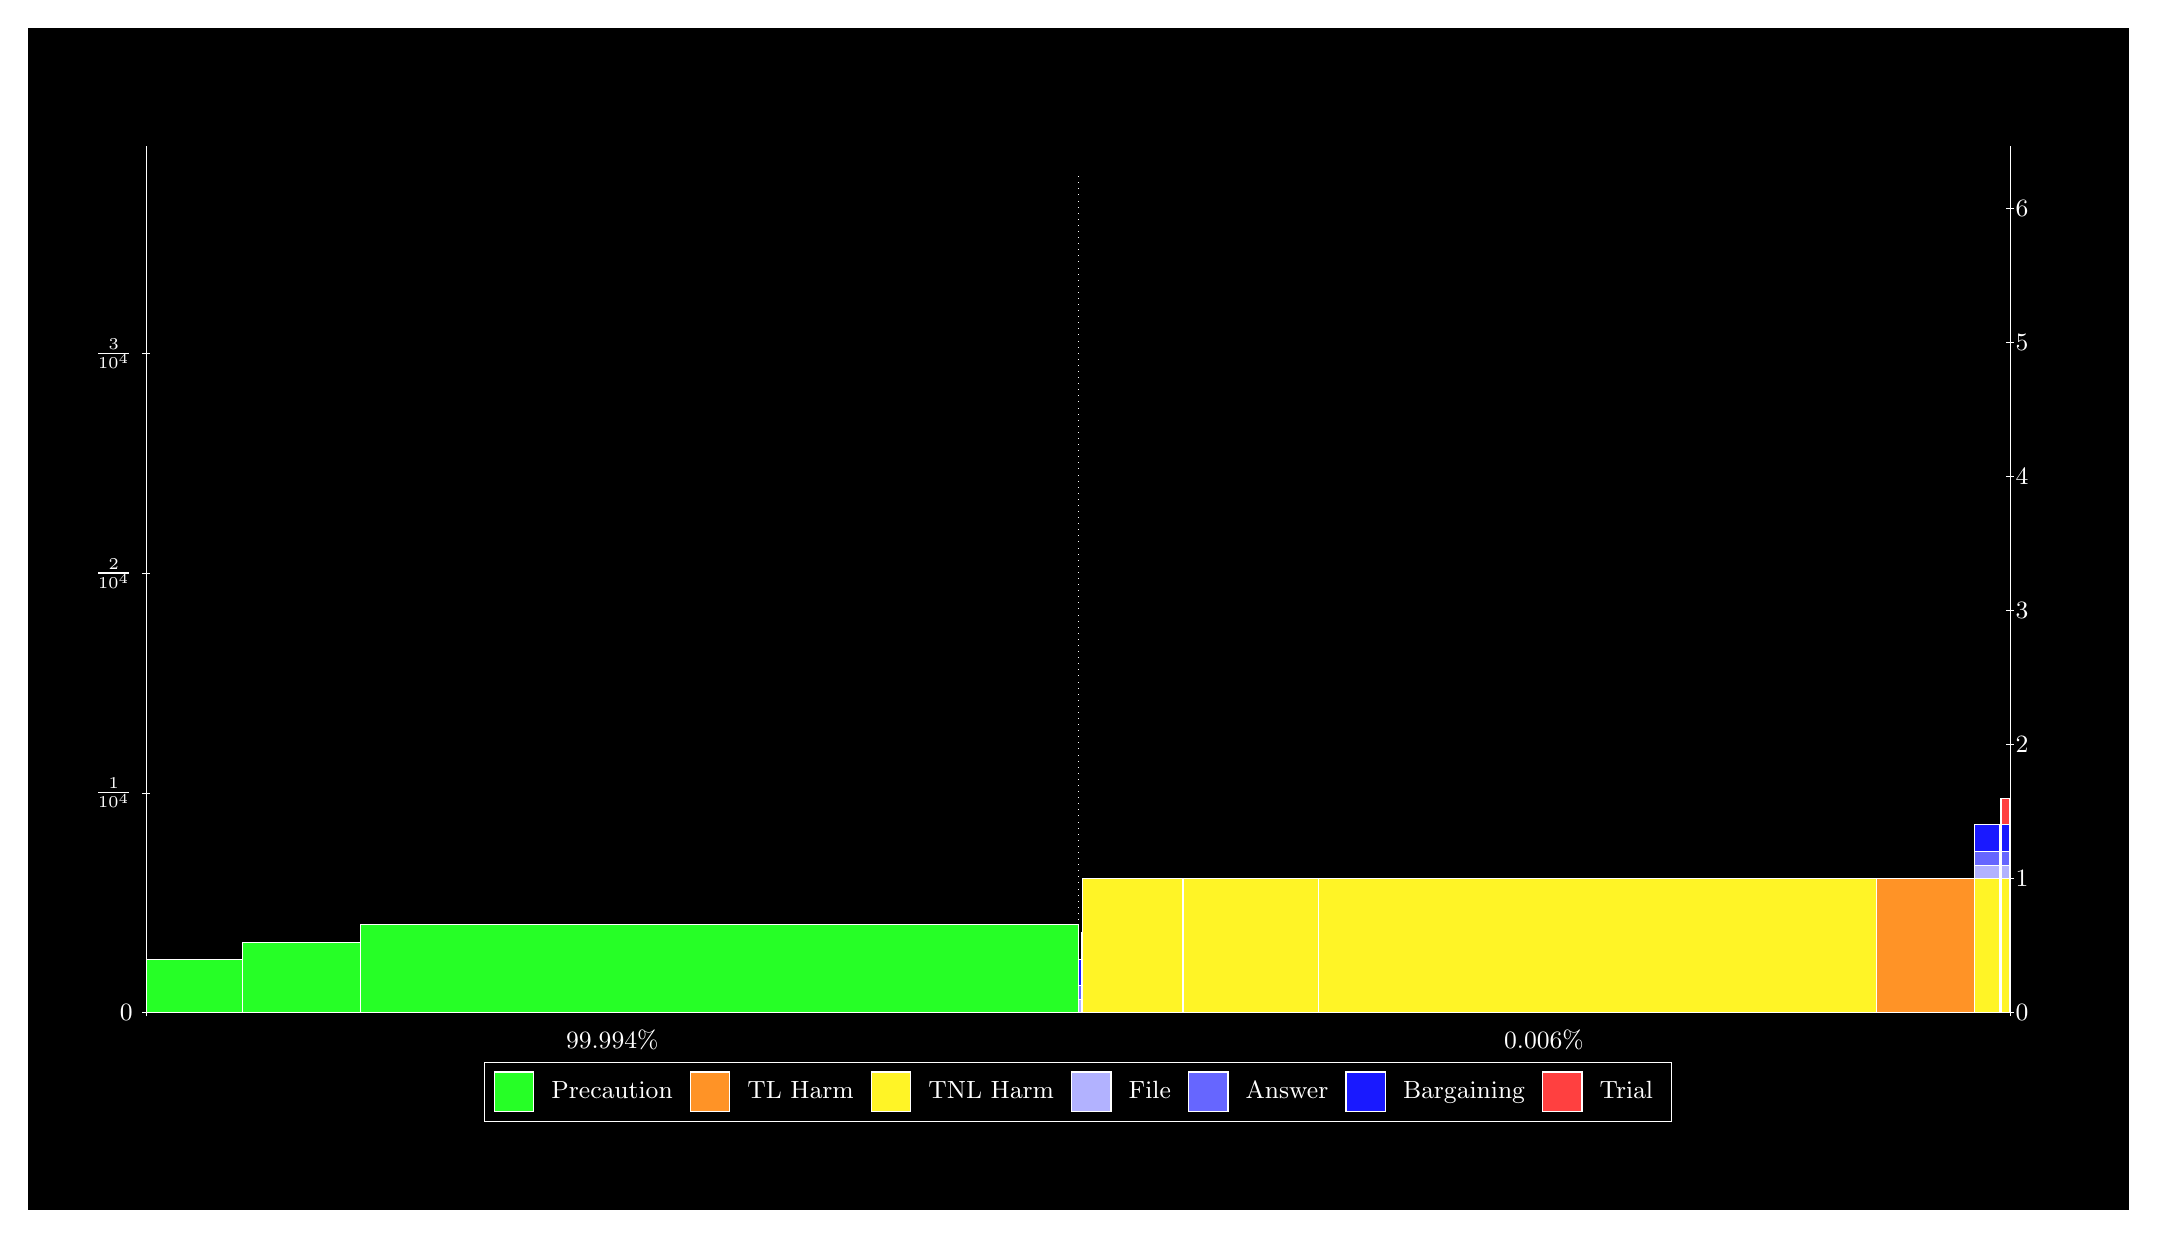
\begin{tikzpicture}
\draw[fill=black] (0,0) rectangle (26.667,15);
\draw[fill=green!85,draw=white,very thin] (1.5,2.5) rectangle (2.7168,3.1693);
\draw[fill=green!85,draw=white,very thin] (2.7168,2.5) rectangle (4.2218,3.3924);
\draw[fill=green!85,draw=white,very thin] (4.2218,2.5) rectangle (13.333,3.6155);
\draw[fill=green!85,draw=white,very thin] (13.333,2.5) rectangle (13.375,2.5);
\draw[fill=blue!30,draw=white,very thin] (13.333,2.5) rectangle (13.375,2.6703);
\draw[fill=blue!60,draw=white,very thin] (13.333,2.6703) rectangle (13.375,2.8406);
\draw[fill=blue!90,draw=white,very thin] (13.333,2.8406) rectangle (13.375,3.1811);
\draw[fill=green!85,draw=white,very thin] (13.375,2.5) rectangle (13.391,2.5001);
\draw[fill=blue!30,draw=white,very thin] (13.375,2.5001) rectangle (13.391,2.6703);
\draw[fill=blue!60,draw=white,very thin] (13.375,2.6703) rectangle (13.391,2.8406);
\draw[fill=blue!90,draw=white,very thin] (13.375,2.8406) rectangle (13.391,3.1811);
\draw[fill=red!75,draw=white,very thin] (13.375,3.1811) rectangle (13.391,3.5217);
\draw[fill=green!85,draw=white,very thin] (13.391,2.5) rectangle (14.662,2.5);
\draw[fill=yellow!85,draw=white,very thin] (13.391,2.5) rectangle (14.662,4.2028);
\draw[fill=green!85,draw=white,very thin] (14.662,2.5) rectangle (14.665,2.5);
\draw[fill=orange!85,draw=white,very thin] (14.662,2.5) rectangle (14.665,4.2028);
\draw[fill=green!85,draw=white,very thin] (14.665,2.5) rectangle (16.389,2.5001);
\draw[fill=yellow!85,draw=white,very thin] (14.665,2.5001) rectangle (16.389,4.2028);
\draw[fill=green!85,draw=white,very thin] (16.389,2.5) rectangle (23.469,2.5001);
\draw[fill=yellow!85,draw=white,very thin] (16.389,2.5001) rectangle (23.469,4.2028);
\draw[fill=green!85,draw=white,very thin] (23.469,2.5) rectangle (24.718,2.5001);
\draw[fill=orange!85,draw=white,very thin] (23.469,2.5001) rectangle (24.718,4.2028);
\draw[fill=green!85,draw=white,very thin] (24.718,2.5) rectangle (25.029,2.5);
\draw[fill=yellow!85,draw=white,very thin] (24.718,2.5) rectangle (25.029,4.2028);
\draw[fill=blue!30,draw=white,very thin] (24.718,4.2028) rectangle (25.029,4.373);
\draw[fill=blue!60,draw=white,very thin] (24.718,4.373) rectangle (25.029,4.5433);
\draw[fill=blue!90,draw=white,very thin] (24.718,4.5433) rectangle (25.029,4.8839);
\draw[fill=green!85,draw=white,very thin] (25.029,2.5) rectangle (25.044,2.5);
\draw[fill=orange!85,draw=white,very thin] (25.029,2.5) rectangle (25.044,4.2028);
\draw[fill=blue!30,draw=white,very thin] (25.029,4.2028) rectangle (25.044,4.373);
\draw[fill=blue!60,draw=white,very thin] (25.029,4.373) rectangle (25.044,4.5433);
\draw[fill=blue!90,draw=white,very thin] (25.029,4.5433) rectangle (25.044,4.8839);
\draw[fill=green!85,draw=white,very thin] (25.044,2.5) rectangle (25.053,2.5);
\draw[fill=yellow!85,draw=white,very thin] (25.044,2.5) rectangle (25.053,4.2028);
\draw[fill=blue!30,draw=white,very thin] (25.044,4.2028) rectangle (25.053,4.373);
\draw[fill=blue!60,draw=white,very thin] (25.044,4.373) rectangle (25.053,4.5433);
\draw[fill=blue!90,draw=white,very thin] (25.044,4.5433) rectangle (25.053,4.8839);
\draw[fill=red!75,draw=white,very thin] (25.044,4.8839) rectangle (25.053,5.2244);
\draw[fill=green!85,draw=white,very thin] (25.053,2.5) rectangle (25.059,2.5);
\draw[fill=orange!85,draw=white,very thin] (25.053,2.5) rectangle (25.059,4.2028);
\draw[fill=blue!30,draw=white,very thin] (25.053,4.2028) rectangle (25.059,4.373);
\draw[fill=blue!60,draw=white,very thin] (25.053,4.373) rectangle (25.059,4.5433);
\draw[fill=blue!90,draw=white,very thin] (25.053,4.5433) rectangle (25.059,4.8839);
\draw[fill=red!75,draw=white,very thin] (25.053,4.8839) rectangle (25.059,5.2244);
\draw[fill=green!85,draw=white,very thin] (25.059,2.5) rectangle (25.163,2.5001);
\draw[fill=yellow!85,draw=white,very thin] (25.059,2.5001) rectangle (25.163,4.2028);
\draw[fill=blue!30,draw=white,very thin] (25.059,4.2028) rectangle (25.163,4.3731);
\draw[fill=blue!60,draw=white,very thin] (25.059,4.3731) rectangle (25.163,4.5433);
\draw[fill=blue!90,draw=white,very thin] (25.059,4.5433) rectangle (25.163,4.8839);
\draw[fill=red!75,draw=white,very thin] (25.059,4.8839) rectangle (25.163,5.2244);
\draw[fill=green!85,draw=white,very thin] (25.163,2.5) rectangle (25.167,2.5001);
\draw[fill=orange!85,draw=white,very thin] (25.163,2.5001) rectangle (25.167,4.2028);
\draw[fill=blue!30,draw=white,very thin] (25.163,4.2028) rectangle (25.167,4.3731);
\draw[fill=blue!60,draw=white,very thin] (25.163,4.3731) rectangle (25.167,4.5433);
\draw[fill=blue!90,draw=white,very thin] (25.163,4.5433) rectangle (25.167,4.8839);
\draw[fill=red!75,draw=white,very thin] (25.163,4.8839) rectangle (25.167,5.2244);
\draw[white,very thin] (1.5,2.5) -- (1.5,13.5);
\draw[white,very thin] (1.45,2.5) -- (1.55,2.5);
\node[font=\small,text=white, anchor=east] at (1.45, 2.5) {0};
\draw[white,very thin] (1.45,5.2887) -- (1.55,5.2887);
\node[font=\small,text=white, anchor=east] at (1.45, 5.2887) {$\frac{1}{10^{4}}$};
\draw[white,very thin] (1.45,8.0773) -- (1.55,8.0773);
\node[font=\small,text=white, anchor=east] at (1.45, 8.0773) {$\frac{2}{10^{4}}$};
\draw[white,very thin] (1.45,10.866) -- (1.55,10.866);
\node[font=\small,text=white, anchor=east] at (1.45, 10.866) {$\frac{3}{10^{4}}$};

\draw[white,dotted,very thin] (13.333,2.83) -- (13.333,13.17);
\draw[white,very thin] (25.167,2.5) -- (25.167,13.5);
\draw[white,very thin] (25.117,2.5) -- (25.217,2.5);
\node[font=\small,text=white, anchor=west] at (25.117, 2.5) {0};
\draw[white,very thin] (25.117,4.2027) -- (25.217,4.2027);
\node[font=\small,text=white, anchor=west] at (25.117, 4.2027) {1};
\draw[white,very thin] (25.117,5.9054) -- (25.217,5.9054);
\node[font=\small,text=white, anchor=west] at (25.117, 5.9054) {2};
\draw[white,very thin] (25.117,7.6082) -- (25.217,7.6082);
\node[font=\small,text=white, anchor=west] at (25.117, 7.6082) {3};
\draw[white,very thin] (25.117,9.3109) -- (25.217,9.3109);
\node[font=\small,text=white, anchor=west] at (25.117, 9.3109) {4};
\draw[white,very thin] (25.117,11.014) -- (25.217,11.014);
\node[font=\small,text=white, anchor=west] at (25.117, 11.014) {5};
\draw[white,very thin] (25.117,12.716) -- (25.217,12.716);
\node[font=\small,text=white, anchor=west] at (25.117, 12.716) {6};

\draw[white,very thin] (1.5,2.5) -- (25.167,2.5);
\draw[white,very thin] (1.5,2.45) -- (1.5,2.55);
\node[font=\small,text=white, anchor=north] at (1.5, 2.45) {};
\draw[white,very thin] (25.167,2.45) -- (25.167,2.55);
\node[font=\small,text=white, anchor=north] at (25.167, 2.45) {};

\node[font=\small,text=white,anchor=south] at (7.4167, 1.9) {99.994\%};
\node[font=\small,text=white,anchor=south] at (19.25, 1.9) {0.006\%};
\draw (13.3333,2.5) node (B) {};
\begin{scope}[align=center]
\matrix[scale=0.5,draw=white,below=0.5cm of B,nodes={draw},column sep=0.1cm]{
\node[rectangle,draw,minimum width=0.5cm,minimum height=0.5cm,fill=green!85]{}; & \node[draw=none,font=\small,text=white]{Precaution}; &
\node[rectangle,draw,minimum width=0.5cm,minimum height=0.5cm,fill=orange!85]{}; & \node[draw=none,font=\small,text=white]{TL Harm}; &
\node[rectangle,draw,minimum width=0.5cm,minimum height=0.5cm,fill=yellow!85]{}; & \node[draw=none,font=\small,text=white]{TNL Harm}; &
\node[rectangle,draw,minimum width=0.5cm,minimum height=0.5cm,fill=blue!30]{}; & \node[draw=none,font=\small,text=white]{File}; &
\node[rectangle,draw,minimum width=0.5cm,minimum height=0.5cm,fill=blue!60]{}; & \node[draw=none,font=\small,text=white]{Answer}; &
\node[rectangle,draw,minimum width=0.5cm,minimum height=0.5cm,fill=blue!90]{}; & \node[draw=none,font=\small,text=white]{Bargaining}; &
\node[rectangle,draw,minimum width=0.5cm,minimum height=0.5cm,fill=red!75]{}; & \node[draw=none,font=\small,text=white]{Trial}; \\\\
};\end{scope}

\end{tikzpicture}
\end{document}